\subsection{Mission}
Nuestra mision aparte de alcanzar el objetivo marcado es atraer usuarios.
El usuario nos busca poco somos unicos, porque le ofrecemos algo que
nadie mas le ofrece, porque somos diferentes. Despuntar entre los demas.
Queremos que el usuario confie en nosotros, nos valores, nos aprecie, que cree un vinculo con nosotros. Para
ello tendremos que cultivar la relacion y ofrecerle un valor que le proporcione satisfaccion.
 
Para lograr esta satisfaccion, tenemos que tener una mision clara, que es lo que ofrecemos, que nos hace diferentes.
Nos podemos plantear cuales son las caracteristicas que otros no tienen, como datos mas actualizados y acurados, 
mayor cobertura de informacion o una funcionalidad que hasta ahora no existe que por ejemplo pueda utilizar la 
informacion que ofrecemos para resolver un problema cotidiano.

Una vez marcada nuestra mision, nos enfrentamos a una serie de problemas, puede que el usario no sepa que 
necesita de esta caracteristica que le proporcionamos. Tenemos un desafio doble, el ofrecerselo a los usuarios y 
el hacerle ver que en realidad es necesario, que le ayuda en su rutina o vida diaria.

Aqui entra en juego el saber aplicar las tecnicas de marketing mas apropiadas para alcanzar a nuestros usuarios.
Tendremos que realizar un estudio de nuestro publico objetivo, que tipo de publicidad consume y por que canal. Asi,
podremos acercanos a ellos de la forma mas adecuada. Lamentablemente, el mercado esta en un cambio continuo,
por lo que dependiendo del momento en el que nos encontramos, deberemos adaptarnos para encontrar la formula 
perfecta.

\subsubsection{How to solve it} 
Deberemos estudiar y analizar que carencias tiene el mercado actualmente y que necesidades tiene el usuario.
Nos plantearemos una serie de preguntas, como pueden ser de que manera puede ayudarme tener este conocimiento.
Definir el publico objetivo, que utiliza en su dia a dia para estar informado o como entretenimiento y buscar
que tipo de publicidad consume para asi poder acercanos a ellos. Hay que tener en cuenta que debemos mantenernos
fiel al espiritu de lo que representamos, por lo que ademas del publico, deberemos saber que tipo de publicidad
se adapta mejor a nuestro producto.

\subsubsection{How we solve it. Aire Guru} 
La mision de Aire Guru es incrementar el concienciamiento de la calidad del Aire. 
Existen varias problematicas respecto a este tema, el primero es la desinformacion del usuario, ya que no es 
consciente de los niveles de poluciones a los que esta expuesto y por otro lado no sabe como le puede perjudiar
a corto o largo plazo.

Aire Guru intenta alertar de la situacion, de una forma que todo el mundo independiente de su nivel cultural 
pueda entender como la calidad del aire nos influye. Pretende poner al alcance de todos el conocimiento sobre
esta problematica. Como de nocivo es vivir en un area altamente contaminada y cuales son las funtes de contaminacion
mas comunes, para que asi, podamos incrementar la concienciacion y poder hacer algo al respecto.


Aire Guru incluye en su glosario las condiciones medicas mas comunes que pueden verse afectadas por la contaminacion
del aire, los agentes contaminantes y las fuentes que provocan estos agentes. Esta acompanado por una iconografia
que refleja cada uno de los sintomas.\\


 \begin{figure}[ht]
    \centering
   \subfigure[Glossary detail]
    {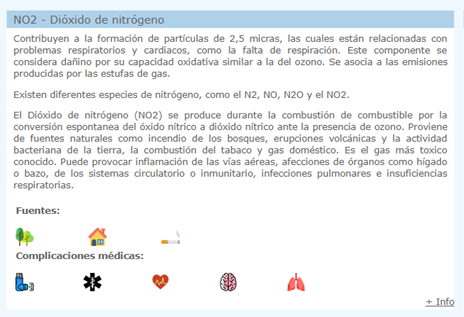
\includegraphics[width=6.2cm  ]{no2_glosary}}
    \hfill
     \subfigure[iconography detail]
     { 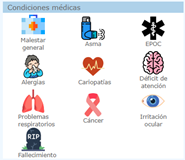
\includegraphics[width=5cm]{iconography}}
  
  \caption{Glossary}
    \end{figure}


\elsparagraph{Evaluation}  
\begin{itemize}
    \done En la encuesta realizada, los usuarios nos comentaron que habia crecido su interes por la contaminacion
    del aire. Algunos de ellos descubrieron que tenian una condicion medica que resulta afectada por la polucion.
    \crossed Aire Guru necesita mas expansion.
    
\end{itemize}
\newpage